\documentclass[a4paper, 12 pt]{article}
\usepackage{graphicx}
\usepackage{float}
\usepackage[portuguese]{babel}
\usepackage{indentfirst}
\usepackage[hidelinks]{hyperref}
\addto\extrasportuguese{\renewcommand{\contentsname}{Sumário}}
\usepackage{amsmath}
\usepackage{amssymb}
\usepackage{parskip}
\usepackage{subcaption}

% Configuração de margens
\usepackage[left=3cm,right=2cm,top=3cm,bottom=2cm]{geometry}

\begin{document}

% Capa
    \begin{center}
    
        
\includegraphics[scale = 0.5]{imgs/FGV_logo.png} 
        
        \textbf{Fundação Getúlio Vargas}\\
        \textbf{Escola de Matemática Aplicada}

        \vspace{2 cm}
        \textbf{Ciência de Redes}

        \vspace{3cm}
        \textbf{Relatório da Simulação de Epidemias}

        \vspace{3 cm}
        \textbf{Anderson Gabriel Falcão dos Santos\\
        Leonardo Alexandre da Silva Ferreira\\
        Ramyro Corrêa Aquines}

        \vspace{3 cm}
        Rio de Janeiro \\
        Novembro / 2025

    \end{center}

% SUMARIO
\newpage
\tableofcontents

\newpage

% CONTEUDO

\section{Introdução}
O estudo da propagação de doenças em redes complexas é fundamental para compreender como a topologia das interações sociais influencia a dinâmica de epidemias. Este relatório apresenta os resultados de simulações numéricas do modelo \textbf{SIS (Suscetível-Infectado-Suscetível)} em dois tipos de topologias de rede: Redes Aleatórias (Erdős-Rényi) e Redes Livre de Escala (Scale-Free).

O objetivo principal é analisar o comportamento da fração de infectados ao longo do tempo variando os parâmetros de infecciosidade ($\beta$) e recuperação ($\mu$), verificar a validade do limiar epidêmico ($R_0$) previsto pela teoria de campo médio e, por fim, estudar a eficácia de diferentes estratégias de imunização.

\section{Metodologia}
As simulações foram realizadas computacionalmente utilizando a biblioteca \textit{NetworkX} para geração dos grafos e algoritmos estocásticos para a dinâmica SIS. Para cada cenário, foram realizadas múltiplas execuções (100 simulações) para obter curvas médias, suavizando as flutuações estocásticas inerentes ao processo.

As redes geradas possuem $N = 10.000$ vértices e grau médio $\langle k \rangle \approx 20$. A condição inicial para todas as simulações foi de 5 vértices infectados escolhidos aleatoriamente.

\section{Simulação em Rede Aleatória (ER)}

Inicialmente, gerou-se uma rede Erdős-Rényi com $N=10000$ e grau médio $\langle k \rangle = 20$. No modelo de campo médio homogêneo, o número básico de reprodução é dado por:
\begin{equation}
    R_0 = \frac{\beta \langle k \rangle}{\mu}
\end{equation}
A teoria prevê que se $R_0 > 1$, a doença se torna endêmica; se $R_0 < 1$, a doença é extinta.

Foram testados três cenários:
\begin{enumerate}
    \item $\beta = 0.02, \mu = 0.1 \Rightarrow R_0 = \frac{0.02 \times 20}{0.1} = 4.0$
    \item $\beta = 0.02, \mu = 0.4 \Rightarrow R_0 = \frac{0.02 \times 20}{0.4} = 1.0$
    \item $\beta = 0.02, \mu = 0.5 \Rightarrow R_0 = \frac{0.02 \times 20}{0.5} = 0.8$
\end{enumerate}

\subsection{Resultados e Discussão}

A Figura \ref{fig:er_simulation} apresenta a evolução temporal da fração de infectados para os três cenários.

\begin{figure}[H]
    \centering
    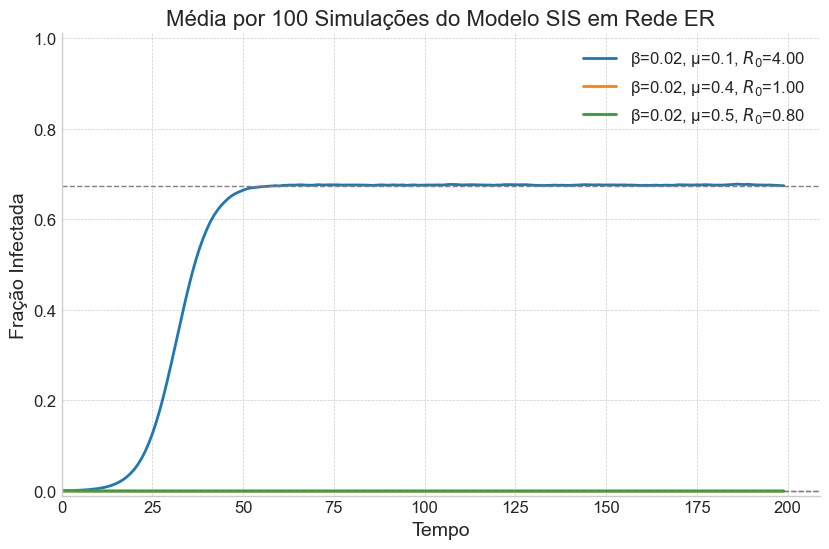
\includegraphics[width=0.9\textwidth]{imgs/q1_img1.png}
    \caption{Evolução temporal da fração de infectados no modelo SIS em uma rede Erdős-Rényi. As curvas representam a média de 100 simulações.}
    \label{fig:er_simulation}
\end{figure}

Observa-se que:
\begin{itemize}
    \item No caso onde $R_0 = 4.0$ (curva azul), a epidemia cresce rapidamente e se estabiliza em um estado endêmico com alta prevalência, confirmando a previsão teórica para $R_0 > 1$.
    \item No caso limítrofe $R_0 = 1.0$ (curva laranja), a doença tem dificuldade em se estabelecer, e caminha para a extinção total.
    \item No caso $R_0 = 0.8$ (curva verde), de maneira similar ao caso anterior, a doença tem dificuldade em se estabelecer, e caminha para a extinção total.
\end{itemize}

\section{Simulação em Rede Livre de Escala (SF)}

Na segunda etapa, utilizou-se uma rede Livre de Escala (gerada via \textit{Configuration Model} seguindo uma distribuição de lei de potência com $\gamma = 2.5$) mantendo $N=10000$ e $\langle k \rangle \approx 20$. 

Os parâmetros testados foram:
\begin{enumerate}
    \item $\beta = 0.01, \mu = 0.1$
    \item $\beta = 0.01, \mu = 0.2$
    \item $\beta = 0.01, \mu = 0.3$
\end{enumerate}

\subsection{Comparação com Rede Aleatória}

A Figura \ref{fig:sf_simulation} exibe os resultados para a rede Livre de Escala.

\begin{figure}[H]
    \centering
    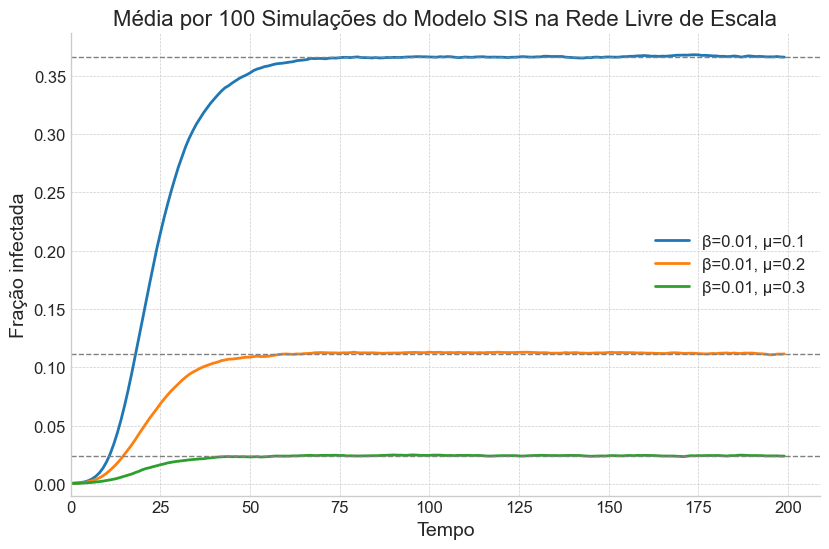
\includegraphics[width=0.9\textwidth]{imgs/q2_img1.png}
    \caption{Evolução temporal da fração de infectados no modelo SIS em uma rede Livre de Escala.}
    \label{fig:sf_simulation}
\end{figure}

Comparando com o modelo ER, as redes livres de escala apresentam uma dinâmica distinta devido à presença de \textit{hubs} (nós muito conectados). Teoricamente, em redes SF com $2 < \gamma \le 3$ e tamanho infinito, o limiar epidêmico tende a zero ($R_0 \to 0$), o que significa que doenças podem persistir mesmo com taxas de infecção muito baixas.

Nas simulações, nota-se que a doença atinge um estado estacionário mais rapidamente ou persiste de forma mais robusta do que em redes homogêneas equivalentes, pois uma vez que os \textit{hubs} são infectados, eles agem como super-espalhadores, sustentando a epidemia.

\section{Estratégias de Imunização e Robustez}

Por fim, analisou-se o impacto da imunização prévia de uma fração $q$ dos vértices na rede Livre de Escala (configuração $\beta=0.01, \mu=0.1$). Foram comparadas três estratégias:
\begin{itemize}
    \item \textbf{Aleatória:} Vértices escolhidos ao acaso.
    \item \textbf{Hubs:} Vértices com maior grau são imunizados primeiro.
    \item \textbf{Vizinhos:} Escolhe-se um nó aleatório e imuniza-se um de seus vizinhos aleatoriamente.
\end{itemize}

\begin{figure}[H]
    \centering
    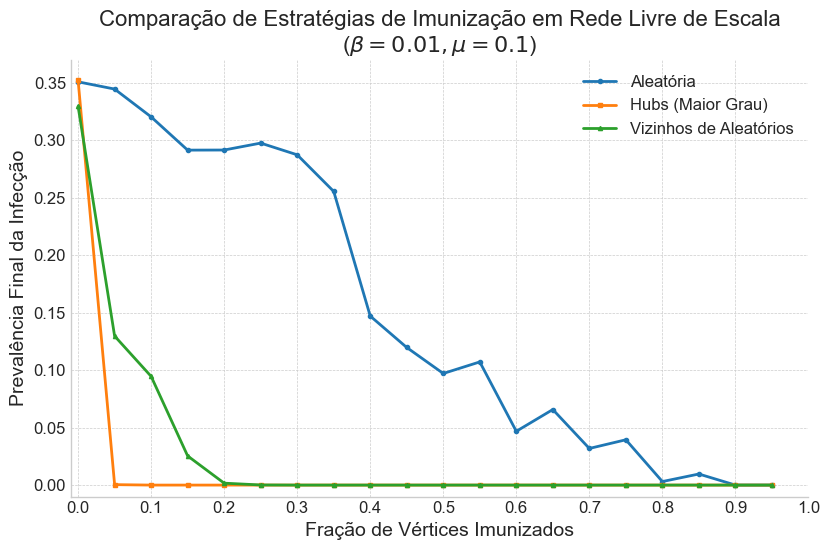
\includegraphics[width=0.9\textwidth]{imgs/q3_img1.png}
    \caption{Prevalência final da epidemia em função da fração de vértices imunizados para diferentes estratégias.}
    \label{fig:imunizacao}
\end{figure}

\subsection{Discussão sobre Robustez}
Os resultados (Figura \ref{fig:imunizacao}) demonstram a relação entre a topologia da rede e sua robustez:

\begin{enumerate}
    \item \textbf{Imunização Aleatória:} A rede SF é extremamente \textbf{robusta a falhas aleatórias}. Mesmo com uma alta fração de vacinados aleatoriamente, a doença continua a se propagar, pois a probabilidade de selecionar e imunizar os \textit{hubs} (que sustentam a conectividade) é estatisticamente baixa.
    
    \item \textbf{Imunização de Hubs:} A rede SF é extremamente \textbf{frágil a ataques direcionados}. Ao imunizar seletivamente os nós de maior grau, a prevalência da doença cai para zero rapidamente com uma fração $q$ muito pequena. Isso fragmenta a rede e remove os super-espalhadores.
    
    \item \textbf{Imunização de Vizinhos:} Esta estratégia se mostra muito mais eficiente que a aleatória e próxima da estratégia de Hubs. Isso ocorre devido ao \textit{Paradoxo da Amizade}: ``seus amigos têm, em média, mais amigos que você". Ao selecionar um vizinho de um nó aleatório, há uma alta probabilidade de encontrar um nó de grau elevado (\textit{hub}) sem precisar conhecer a topologia global da rede.
\end{enumerate}

\section{Conclusão}
As simulações confirmaram que a estrutura da rede altera drasticamente a dinâmica epidêmica. Enquanto em redes homogêneas (ER) o limiar $R_0$ clássico prevê bem a transição de fase, em redes heterogêneas (SF) a presença de hubs facilita a persistência da doença. Consequentemente, estratégias de imunização focadas na topologia (como a vacinação de hubs ou vizinhos) são ordens de grandeza mais eficientes do que a vacinação em massa aleatória para conter epidemias em redes livres de escala.

\end{document}